% Uebung Nr. 7 kompensierter Spannungsteiler nach Brinkmeyer
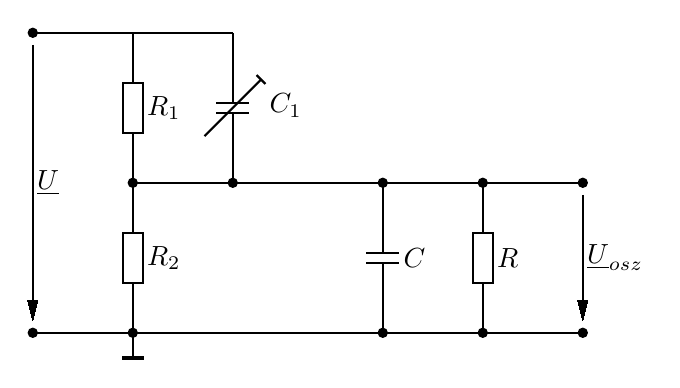
\begin{tikzpicture}[scale=2.54]%
% dpic version 2024.01.01 option -g for TikZ and PGF 1.01
\ifx\dpiclw\undefined\newdimen\dpiclw\fi
\global\def\dpicdraw{\draw[line width=\dpiclw]}
\global\def\dpicstop{;}
\dpiclw=0.8bp
\dpiclw=0.8bp
\dpicdraw[fill=black](0,0) circle (0.007874in)\dpicstop
\dpicdraw[fill=black](0,-1.5) circle (0.007874in)\dpicstop
\filldraw[line width=0bp](-0.025,-1.34)
 --(0,-1.44)
 --(0.025,-1.34) --cycle\dpicstop
\dpicdraw (0,-0.06)
 --(0,-1.417094)\dpicstop
\draw (0,-0.75) node[right=-2bp]{$ \underline{U}$};
\dpicdraw (0,0)
 --(0.5,0)\dpicstop
\dpicdraw (0.5,0)
 --(0.5,-0.25)\dpicstop
\dpicdraw (0.5,-0.5)
 --(0.55,-0.5)
 --(0.55,-0.25)
 --(0.45,-0.25)
 --(0.45,-0.5)
 --(0.5,-0.5)\dpicstop
\dpicdraw (0.5,-0.5)
 --(0.5,-0.75)\dpicstop
\draw (0.55,-0.375) node[right=-2bp]{$ R_1$};
\dpicdraw[fill=black](0.5,-0.75) circle (0.007874in)\dpicstop
\dpicdraw (0.5,-0.75)
 --(0.5,-1)\dpicstop
\dpicdraw (0.5,-1.25)
 --(0.55,-1.25)
 --(0.55,-1)
 --(0.45,-1)
 --(0.45,-1.25)
 --(0.5,-1.25)\dpicstop
\dpicdraw (0.5,-1.25)
 --(0.5,-1.5)\dpicstop
\draw (0.55,-1.125) node[right=-2bp]{$ R_2$};
\dpicdraw[fill=black](0.5,-1.5) circle (0.007874in)\dpicstop
\dpicdraw (0.5,-1.5)
 --(0.5,-1.625)\dpicstop
\dpicdraw[line width=1.6bp](0.555556,-1.625)
 --(0.444444,-1.625)\dpicstop
\dpicdraw (0.5,0)
 --(1,0)\dpicstop
\dpicdraw (1,0)
 --(1,-0.35)\dpicstop
\dpicdraw (0.916667,-0.35)
 --(1.083333,-0.35)\dpicstop
\dpicdraw (0.916667,-0.4)
 --(1.083333,-0.4)\dpicstop
\dpicdraw (1,-0.4)
 --(1,-0.75)\dpicstop
\dpicdraw (0.858579,-0.516421)
 --(1.141421,-0.233579)\dpicstop
\dpicdraw (1.119324,-0.211482)
 --(1.163518,-0.255676)\dpicstop
\draw (1.163518,-0.363951) node[right=-2bp]{$ C_1$};
\dpicdraw[fill=black](1,-0.75) circle (0.007874in)\dpicstop
\dpicdraw (1,-0.75)
 --(0.5,-0.75)\dpicstop
\dpicdraw (1,-0.75)
 --(1.75,-0.75)\dpicstop
\dpicdraw[fill=black](1.75,-0.75) circle (0.007874in)\dpicstop
\dpicdraw (1.75,-0.75)
 --(1.75,-1.1)\dpicstop
\dpicdraw (1.666667,-1.1)
 --(1.833333,-1.1)\dpicstop
\dpicdraw (1.666667,-1.15)
 --(1.833333,-1.15)\dpicstop
\dpicdraw (1.75,-1.15)
 --(1.75,-1.5)\dpicstop
\draw (1.833333,-1.125) node[right=-2bp]{$ C$};
\dpicdraw[fill=black](1.75,-1.5) circle (0.007874in)\dpicstop
\dpicdraw (1.75,-0.75)
 --(2.25,-0.75)\dpicstop
\dpicdraw[fill=black](2.25,-0.75) circle (0.007874in)\dpicstop
\dpicdraw (2.25,-0.75)
 --(2.25,-1)\dpicstop
\dpicdraw (2.25,-1.25)
 --(2.3,-1.25)
 --(2.3,-1)
 --(2.2,-1)
 --(2.2,-1.25)
 --(2.25,-1.25)\dpicstop
\dpicdraw (2.25,-1.25)
 --(2.25,-1.5)\dpicstop
\draw (2.3,-1.125) node[right=-2bp]{$ R$};
\dpicdraw[fill=black](2.25,-1.5) circle (0.007874in)\dpicstop
\dpicdraw (2.25,-0.75)
 --(2.75,-0.75)\dpicstop
\dpicdraw[fill=black](2.75,-0.75) circle (0.007874in)\dpicstop
\dpicdraw[fill=black](2.75,-1.5) circle (0.007874in)\dpicstop
\filldraw[line width=0bp](2.725,-1.34)
 --(2.75,-1.44)
 --(2.775,-1.34) --cycle\dpicstop
\dpicdraw (2.75,-0.81)
 --(2.75,-1.417094)\dpicstop
\draw (2.75,-1.125) node[right=-2bp]{$ \underline{U}_{osz}$};
\dpicdraw (2.75,-1.5)
 --(0,-1.5)\dpicstop
\end{tikzpicture}%
